% Aquí empieza la clase 4

\begin{teo}[Teorema de la función implícita, generalización de la versión 3]
    Sea $F: \R^{n+m} \rightarrow \R^m$ diferenciable y de clase $C^2$, donde $F = (F_1, \dots, F_m)$ y a su vez $F_i(x_1, \dots, x_n, z_1, \dots, z_m)$. Consideremos $p_0 = (x_0, z_0) \in \R^{n+m}$. Consideremos también para cada $i = 1, \dots m$, $\Delta$ de la siguiente manera
    
    \[
    \Delta =
    \renewcommand\arraystretch{2}
    \begin{vmatrix}
        \frac{\partial F_1}{\partial z_1} & \dots & \frac{\partial F_1}{\partial z_m} \\
        \vdots & \ddots & \vdots \\
        \frac{\partial F_m}{\partial z_1} & \dots & \frac{\partial F_m}{\partial z_m}
    \end{vmatrix}
    \]
    
    \noindent donde cada derivada está evaluada en el punto $p_0$.
    
    Si tenemos que $F(p_0) = 0$ y $\Delta(p_0) \neq 0$, entonces en un entorno de $p_0$ tendremos que el sistema
    
    \[
    \begin{cases}
        F_1(x_1, \dots, x_n, z_1, \dots, z_m) = 0 \\
        \vdots \\
        F_m(x_1, \dots, x_n, z_1, \dots, z_m) = 0
    \end{cases}
    \]
    
    \noindent define de forma implícita a las funciones $z_i = f_i(x_1, \dots, x_n)$ con $i = 1, \dots, m$.
    
    Además, tendremos para $k = 1, \dots, n$ y $j = 1, \dots, m$
    
    \[
    \dfrac{\partial z_j}{\partial x_k} = -\dfrac{\dfrac{\partial(F_1, \dots, F_m)}{\partial(z_1, \dots, z_{j-1}, x_k, \dots, z_m)}}{\dfrac{\partial(F_1, \dots, F_m)}{\partial(z_1, \dots, z_m)}}
    \]
\end{teo}

A continuación no demostraremos este último teorema porque los cálculos se hacen muy extensos, pero si discutiremos algunas aplicaciones del T.F.I.:

\begin{ejem}
    Sean una función $F: \R^3 \rightarrow \R$ y $p_o = (x_0, y_0, z_0)$ tal que $F(p_0) = 0$. Sean también $\partial_xF$, $\partial_yF$ y $\partial_zF$ continuas en un entorno de $p_0$. Entonces $F(x,y,z) = 0$ define implícitamente $z = f(x,y)$. Más aún, se puede decir que
    
    \[
    \frac{\partial z}{\partial x}(p_0) = - \frac{\partial_xF(p_0)}{\partial_zF(p_0)}
    \qquad
    \frac{\partial z}{\partial y}(p_0) = - \frac{\partial_yF(p_0)}{\partial_zF(p_0)}
    \]
    
    \noindent si $\partial_zF(p_0) \neq 0$.
    
    Entonces, si calculamos la ecuación del plano tangente, esta nos queda como
    
    \begin{align*}
        z - z_0 &= \frac{\partial f}{\partial x}(x_0,y_0)(x-x_0) + \frac{\partial f}{\partial y}(x_0,y_0)(y-y_0) \\
            &= \partial_zF(p_0)(z-z_0) + \partial_yF(p_0)(y-y_0) + \partial_xF(p_0)(x-x_0) = 0
    \end{align*}
\end{ejem}

\begin{ejem}
    También es muy utilizado en el estudio de las ecuaciones diferenciales ordinarias exactas. Este tema lo abordaremos más adelante.
\end{ejem}

\subsection{Teorema de la función inversa}
\stepcounter{subsec}

Este teorema al igual que el teorema de la función implícita es central en el curso de análisis. Se irá desarrollando poco a poco porque la demostración es bien extensa.

Primero, veremos un lema que además de ser muy útil para la demostración de este teorema, también se utiliza en la materia de ecuaciones diferenciales.

\begin{lem}[Lema de contracción]\label{lem:4.1.1}
    Sean $M \subseteq \R^n$ cerrado y $F: M \rightarrow M$ una función y $K \in (0,1)$ tales que
    
    \[
    \normaeuc{F(x) - F(y)} \leq K\normaeuc{x - y} \quad \forall x,y \in M
    \]
    
    Entonces $F$ tiene un $x_0 \in M$ tal que $F(x_0) = x_0$. Luego nos queda que la sucesión $\sucinf{F^n(x_0)}{n}$ es de Cauchy y converge a $x_0$.
\end{lem}

\begin{proof}
    Primero tenemos que por hipótesis, para cada $x \in M$ fijo y arbitrario
    
    \[
    \normaeuc{F^2(x) - F(x)} = \normaeuc{F(F(x)) - F(x)} \leq K\normaeuc{F(x) - x}
    \]
    
    Ahora, por inducción podemos decir que
    
    \[
    \normaeuc{F^{n+1}(x) - F^n(x)} \leq K\normaeuc{F^n(x) - F^{n-1}(x)} \leq K^n\normaeuc{F(x) - x}
    \]
    
    En lo particular esto nos dice que $\sucinf{F^n(x_0)}{n}$ es una sucesión acotada, ya que
    
    \begin{align*}
        \normaeuc{F^n(x) - x} &\leq \normaeuc{F^n(x) - F^{n-1}(x)} + \normaeuc{F^{n-1}(x) - F^{n-2}(x)} + \dots \normaeuc{F(x) - x} \\
            &\leq \LaTeXunderbrace{(K^{n-1} + K^{n-2} + \dots + K)}_{\text{converge a $\frac{1}{1-K}$}}\normaeuc{F(x) - x}
    \end{align*}
    
    Nuevamente por inducción tenemos que para $m,k \in \N$
    
    \[
    \normaeuc{F^{m+k}(x) + F^m(x)} \leq K^m\normaeuc{F^k(x) + x}
    \]
    
    Ahora, como el término $F^k(x) - x$ está acotado, entonces existe $N_0 \in \N$ tal que $n,m \geq N_0$ con $n = m+k$, entonces
    
    \[
    \text{si $m,m \geq N_0$} \quad \implies \quad \normaeuc{F^{m+k}(x) + F^m(x)} < \varepsilon
    \]
    
    \noindent esto lo podemos hacer porque $\limtoinfty{m}{k^m} = 0$ ya que $K \in (0,1)$.
    
    Por lo tanto, $\sucinf{F^n(x_0)}{n}$ es de Cauchy.
    
    Ahora sea $x_0 \in M$ tal que $x_0 = \limtoinfty{n}{F^n(x)}$. Entonces dado $\varepsilon > 0$, existe $N_1$ tal que
    
    \[
    \text{si $n \geq N_1$} \quad \implies \quad \normaeuc{x_0 - F^n(x)} < \varepsilon
    \]
    
    Por lo tanto, si $n \geq N_1$
    
    \[
    \normaeuc{F(x_0) - F^{n+1}(x)} \leq K\normaeuc{x_0 - F^n(x)} < K\varepsilon
    \]
    
    De esta manera, $\limtoinfty{n}{F^n(x)} = F(x_0)$. En consecuencia $F(x_0) = x_0$.
    
    Lo único que queda es ver que $x_0$ es único: Supongamos que existe $x_1 \in M$ tal que $F(x_1) = x_1$. Consideremos ahora lo siguiente
    
    \begin{align*}
        \normaeuc{x_0 - x_1} &= \normaeuc{F(x_0) - F(x_1)} \leq K\normaeuc{x_0 - x_1} \\
        &\implies \normaeuc{x_0 - x_1} < K\normaeuc{x_0 - x_1}
    \end{align*}
    
    \noindent con $K \in (0,1)$. Esto es una contradicción ya que $\normaeuc{x_0 - x_1} > K\normaeuc{x_0 - x_1}$. Luego no existe dicho $x_1$ y concluimos que $x_0$ es único.
    
    Y así queda demostrado el lema de contracción, que próximamente utilizaremos para la demostración del lema de la función implícita.
\end{proof}

Ahora podemos presentar el teorema de la función inversa. Recordar que de este teorema existen muchas versiones. En este curso nos centraremos en una sola.

\begin{teo}[Teorema de la función inversa]\label{teo:inversa}
    Sean $A \subset \R^n$ abierto, conexo y convexo. Sea $p_0 \in A$, $F: A \rightarrow \R^n$ de clase $C^1(A)$. Supongamos que $JF(p_0) \neq 0$.
    
    Entonces $F$ es $C^1$ invertible localmente en un entorno de $p_0$ y si $G$ es su inversa local, tenemos que $y = G(x)$ y $JG(y) = [JF(x)]^{-1}$.
\end{teo}

\begin{figure}
    \centering
    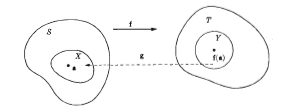
\includegraphics{img/funcion-inversa.PNG}
    \caption{Situación descrita en el teorema de la función inversa.}
\end{figure}

\begin{proof}
    Primero, denotaremos
    
    \[
    \lambda = JF(p_0)
    \]
    
    \noindent así, $\lambda$ define una transformación de $\R^n \rightarrow \R^n$ lineal, continua e invertible. 
    
    Sea ahora $\lambda^{-1} \cdot F(x)$\marginfootnote{No confundir, esto se refiere a la composición.}, derivando nos queda que
    
    \[
    \left( \lambda^{-1} \cdot F(x) \right)' = \lambda^{-1}JF(x)
    \]
    
    \noindent y si $x = p_0$ entonces
    
    \[
    \lambda^{-1}JF(p_0) = \lambda^{-1}\lambda = id
    \]
    
    Entonces, si obtenemos que $\lambda^{-1} \cdot F$ es localmente invervtible, concuimos que $F$ también lo es (ya que $F = \lambda\lambda^{-1}F$). Esto reduce el teorema al caso en que $JF(p_0) = id$.
    
    Sea ahora $q_0 = F(p_0)$ y $H(x) = F(x + p_0) - q_0$ (vemos que $H(0) = 0$). Por lo tanto, $H$ está definida en un abierto que contiene al valor $0$, ya que $F$ está definida en un abierto que contiene a $p_0$. Entonces bastará demostrar que $H$ es invertible (localmente) alrededor de $0$.
    
    Bajo todas estas consideraciones, bastará demostrar el teorema bajo tres simplificaciones relevantes:
    
    \[
    p_0 = 0, \qquad F(0) = 0, \qquad JF(0) = id
    \]
    
    % Aquí empieza la clase 5
    Sea $W(x) = x - F(x)$ donde $JW(x) = I - JF(x)$. Vemos que $JW(0) = 0$. Por continuidad de $F$, existe un valor $r > 0$ tal que
    
    \begin{equation}\label{eq:5.1.1}
        \text{si $\normaeuc{x} < 2r$} \quad \implies \quad \normap{JW(x)}{} \leq \frac{1}{2}
    \end{equation}
    
    \noindent donde $\normap{JW(x)}{} = \sup_{\normaeuc{u} \leq 1} \normaeuc{JW(x) \cdot u}$.
    
    Consideremos ahora $\psi(t) = W(c(t))$, donde $c(t) = tx + (1-t)0$ con $t \in [0,1]$ (en $c(0) = 0$ y en $c(1) = x$). Con esta parametrización, podemos aplicar \TVM~y existe $t_0 \in (0,1)$ tal que
    
    \begin{equation}\label{eq:5.1.2}
        \psi'(t_0) = \psi(1) - \psi(0)
    \end{equation}
    
    Ahora, por un lado tenemos que
    
    \[
    \psi'(t) = JW\left(c(t)\right)x \implies \psi'(t_0) = JW\left(c(t_0)\right)x
    \]
    
    Entonces $\psi(1) = W(x)$ y $\psi(0) = W(0) = 0$. Y por \ref{eq:5.1.1} y \ref{eq:5.1.2} tenemos que
    
    \begin{align*}
        \normaeuc{\psi(t_0)} &\leq \normaeuc{x}\normap{JW\Big( c(t_0) \Big)}{} \\
            &\leq \frac{\normaeuc{x}}{2}
    \end{align*}
    
    Esto nos permite concluir que $\normaeuc{W(x)} \leq \normaeuc{x}/2$. ¿Qué nos está diciendo esto? Que $W$ está definida de esta manera
    
    \[
    W: \overline{B(0,r)} \rightarrow \overline{B(0,r/2)} \quad \text{y} \quad W\left( B(0,r) \right) = B(0, r/2)
    \]
    
    Con la función así definida, ahora queremos asegurar que para dado $y \in \overline{B(0, r/2)}$, existe un único $x \in \overline{B(0,r)}$ tal que $F(x) = y$. Sea ahora $W_y(x) = y + W(x)$. Entonces aplicando nuevamente el \TVM~tendremos lo siguiente:
    
    \begin{align*}
        \normaeuc{W_y(x_1) - W_y(x_2)} &= \normaeuc{y + W(x_1) - y - W(x_2)} = \normaeuc{W(x_1) - W(x_2)} \\
            &\leq \frac{1}{2}\normaeuc{x_1 - x_2}
    \end{align*}
    
    \noindent con $x_1, x_2 \in \overline{B(0,r)}$. Al igual que antes, esto lo logramos con la ayuda de una función auxiliar $\psi(t) = W\left( c(t) \right)$ donde $c(t) = (1-t)x_1 + tx_2$ (con $t \in (0,1)$).
    
    De esta forma, estamos concluyendo que
    
    \[
    \normaeuc{W_y(x_1) - w_y(x_2)} \leq \frac{1}{2} \normaeuc{x_1 - x_2}, \qquad \forall x_1, x_2 \in \overline{B(0,r)}
    \]
    
    Y aplicando el \LC~, se sigue que $W_y$ tiene un único punto fijo $x$ tal que $W_y(x) = x$. Entonces esto implica que
    
    \begin{align*}
        x = y + W(x) \quad &\implies \quad x = y + x - F(x) \\
            &\implies \quad F(x) = y
    \end{align*}
    
    \noindent para un único valor $x \in \overline{B(0,r/2)}$.
    
    Ahora demostremos la otra parte del teorema. Consideremos el conjunto abierto
    
    \[
    U_1 = \{ x \in B(0,r) : \normaeuc{F(x)} < r/2\}
    \]
    
    Sea $V_1 = F(U_1)$. Así, $F: U \rightarrow V_1$ es inyectiva y podemos construir $G$ tal que $G: V_1 \rightarrow U_1$. Queremos ahora asegurar que $V_1$ es abierto y $G \in C^1$: Sea $x_1$ tal que $y_1 = F(x_1)$ con $\normaeuc{y_1} < r/2$. Sea también $y \in \R^n$ tal que $\normaeuc{y} < r/2$. Entonces hay un único $x \in \overline{B(0,r)}$ tal que $F(x) = y$ y expresando $x = x - F(x) - F(x)$, tendremos que
    
    \begin{align*}
        x - x_1 &= x - F(x) + F(x) - x_1 + F(x_1) - F(x_1) \\
            &= F(x) - F(x_1) + W(x) - W(x_1)
    \end{align*}
    
    Y tomando la norma, nos queda por desigualdad triangular lo siguiente
    
    \begin{align*}
        \normaeuc{x - x_1} &\leq \normaeuc{F(x) - F(x_1)} + \normaeuc{W(x) - W(x_1)} \\
            &\leq \normaeuc{F(x) - F(x_1)} + \frac{\normaeuc{x - x_1}}{2}
    \end{align*}
    
    De aquí obtenemos la siguiente desigualdad
    
    \begin{equation}\label{eq:5.1.3}
        \frac{\normaeuc{x-x_1}}{2} \leq \normaeuc{F(x_1) - F(x_2)}
    \end{equation}
    
    Así, si $y, y_1$ son cercanos entonces $x, x_1$ son también son cercanos. Por lo tanto, tenemos que por un lado
    
    \[
    \normaeuc{x} < r \wedge \normaeuc{F(x)} < \frac{r}{2} \quad \implies \quad x \in U_1 \text{~y por lo tanto $y \in V_1$}
    \]
    
    Esto nos dice que $B(0, r/2) \subset V_1$ y esto implica que $V_1$ es abierto en $\R^n$.
    
    Por otro lado, la desigualdad \ref{eq:5.1.3} implica que
    
    \[
    \frac{\normaeuc{G(y) - G(y_1)}}{2} \leq \normaeuc{y_1 - y}
    \]
    
    Y ahora se puede decir lo siguiente: Dado $\varepsilon > 0$, existe $\delta > 0$ tal que si $\delta > \varepsilon / 2$ entonces concluimos que $G$ es continua.
    
    Para demostrar que $G$ es diferenciable, recordemos que como $JF(x_1)$ es invertible, entonces podemos expresar
    
    \[
    F(x) - F(x_1) = JF(x_1)(x-x_1) + \Phi(x-x_1)(x-x_1)
    \]
    
    \noindent donde $\Phi$ es tal que $\lim_{x \to x_1} \Phi(x-x_1) = 0$. Esto se deduce de la definición de diferenciabilidad.
    
    Ahora, podemos calcular el siguiente factor
    
    \begin{align*}
        G(y) - G(y_1) &- \Big( JF(x_1) \Big)^{-1}(y-y_1) \\
            &= (x-x_1) - \Big( JF(x_1) \Big)^{-1}\Big( F(x) - F(x_1) \Big) \\
            &= (x-x_1) - \Big( JF(x_1) \Big)^{-1}\Big( JF(x_1)(x-x_1) + \Phi(x-x_1)(x-x_1) \Big) \\
            &= \Big( JF(x_1) \Big)^{-1}\Phi(x-x_1)(x-x_1) \\
            &= \Big( JF(x_1) \Big)^{-1}\Big( \Phi\big( G(y) - G(y_1) \big)(y-y_1) \Big)
    \end{align*}
    
    Luego,
    
    \[
    \normaeuc{G(y) - G(y_1) - [JF(x_1)]^{-1}(y-y_1)} \leq \normap{JF^{-1}(x_1)}{}\normaeuc{x-x_1}\normaeuc{\Phi(x-x_1)}
    \]
    
    Y por la desigualdad \ref{eq:5.1.3}, lo anterior nos queda como
    
    \[
    \normaeuc{G(y) - G(y_1) - [JF(x_1)]^{-1}(y-y_1)} \leq 2C\normaeuc{y_1 - y}\normaeuc{\Big( G(y_1) - G(y) \Big)}
    \]
    
    Como $G$ es continua, $y \to y_1$ entonces $G(y) \to G(y_1)$ y $\lim_{x \to x_1} \Phi(x-x_1) = 0$ entonces podemos acotar el factor $\normaeuc{\Big( G(y_1) - G(y) \Big)}$ por otro tan pequeño como queramos. Luego dado $\varepsilon > 0$, $\exists \delta_0 > 0$ tal que
    
    \[
    \text{si $\normaeuc{y - y_1} < \delta_0$} \quad \implies \quad \normaeuc{\Big( G(y_1) - G(y) \Big)} < \frac{\varepsilon}{2C}
    \]
    
    Por lo tanto, si $\normaeuc{y - y_1} < \delta_0$ entonces
    
    \[
    \dfrac{\normaeuc{G(y) - G(y_1) - [JF(x_1)]^{-1}(y-y_1)}}{\normaeuc{y - y_1}} \leq \varepsilon
    \]
    
    En conclusión estamos diciendo que $G$ es diferenciable y además $JG(y_1) = [JF(x_1)]^{-1}$.
    
    Y así queda demostrado el teorema de la función inversa.
\end{proof}